\begin{remark}
    Section made from lectures done by Lindis Bjoland. Other sources are \citet{1995Itsp} --- parts of chapter 14 --- \& \citet{BrekkeAsgeir2013Potu} --- chapter 6.8 and chapter 7 part 11 to 12.
\end{remark}
\textbf{Plan for the week}
\begin{enumerate}[\(\bullet \)]
    \item \emph{Monday} --- Introduction about auroral emissions
    \item \emph{Tuesday} --- Particle precipitation
    \item \emph{Wednesday} --- Auroral distribution in space/time
    \item \emph{Friday} --- Exercises/info.\ about field work
\end{enumerate}
High energy particles may use 20 mins to reach the Earth, while the solar wind takes 2--4 days.\\

\begin{minipage}{.49\linewidth}
\textbf{Dayside}
    \begin{enumerate}[\(\triangleright \)]
    \item source is the solar wind
    \item soft precipitation (\(<\SI{1}{\kilo\electronvolt}\))
    \item mainly red emission
    \item high peak emission height
\end{enumerate}\end{minipage}
\begin{minipage}{.49\linewidth}
\textbf{Nightside}
\begin{enumerate}[\(\triangleright \)]
    \item source is the magnetotail
    \item hard precipitation (\(1-\SI{15}{\kilo\electronvolt}\))
    \item mainly green emission
    \item low peak emission height
\end{enumerate}\end{minipage}

\section{Auroral emissions}
\textbf{E.g.:} Forbidden transition of \(\SI{5577}{\angstrom}\) \\
\([OI]~2p^4\prescript{1}{}{D}-2p^4\prescript{1}{}{S}\) where \([~]\) denote a forbidden transition.
\begin{equation*}
    \underset{\substack{\uparrow \\ \tn{shell}}}{2}\underset{\substack{\uparrow \\ \tn{orbital}}}{p}^4
\end{equation*}
where \(4\) here denotes the number of electrons.
\begin{enumerate}[\(\bullet \)]
    \item \(n=2\): principal quantum number
    \item \(\ell \): azimuthal quantum number (\(\ell=0, 1, 2, \ldots , (n-1)\))
    \item \(\prescript{1}{}{D}/\prescript{1}{}{S}\): two terms in the ground configurations with multiplicity \(2S+1\)
    \item I\@: unionized
    \item II\@: singly ionized
\end{enumerate}
Dissipation in the ionosphere: \begin{enumerate}
    \item excitation \(\Rightarrow \) auroral emissions
    \item ionization \(\Rightarrow \) enhancement of conductivity
    \item collisions/heating
\end{enumerate}

\subsection{Cross section}
The cross section is used to described the likelihood of a favorable collision. In the high energy tail there will be particles that need to loose energy before they are able to excite, and each ion behave differently. The cross section will decrease towards higher energies from the maximum as can be seen in \cref{fig:L4_cross_section}.
\begin{figure}[t]
    \centering
    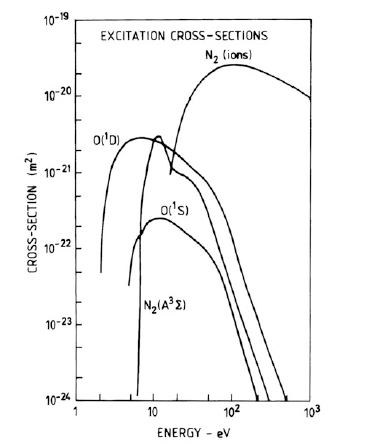
\includegraphics[width=.6\linewidth]{bilder/L4_cross_section.png}
    \caption{}\label{fig:L4_cross_section}
\end{figure}

\subsection{Atomic oxygen energy levels}
The difference in excitation energy implies that the intensity ratio between green (\(\SI{5577}{\angstrom}\)) and red (\(\SI{6300}{\angstrom}\)) emission decreases with decreasing energy of precipitating particles. We end up with, when looking at the intensities of the light, the fraction
\begin{equation*}
    \frac{I(\SI{5577}{\angstrom})}{I(\SI{6300}{\angstrom})}=\frac{\tn{green}}{\tn{red}}
\end{equation*}
which takes in the intensities of the two wavelengths. As mentioned, this will decrease with decreasing energy of the electrons. This means that lower energy will give a greater chance of red light.
Impact excitation
\begin{equation*}
    \tn{O}(\prescript{3}{}{P})+e\rightarrow \tn{O}(\prescript{1}{}{S})+e
\end{equation*}
followed by an emission of either \(\SI{5577}{\angstrom}\) or \(\SI{2972}{\angstrom}\). Red doublet is described by
\begin{equation*}
    \tn{O}(\prescript{3}{}{P})+e\rightarrow \tn{O}(\prescript{1}{}{D})+e
\end{equation*}
followed by emission of the red line
\begin{equation*}
    \tn{O}(\prescript{1}{}{D})\rightarrow
\end{equation*}
\begin{equation*}
    \boxed{\SI{1}{\electronvolt}=\num{1.602e-19}\si{\joule},\quad E=h\nu=\frac{hc}{\lambda} [\si{\joule}]}
\end{equation*}

\subsection{Oxygen emission}
The {\color{red}red} color at \(\lambda\approx\SI{6300}{\angstrom}\) has its peak at \(\sim\SI{230}{\kilo\metre}\). It comes from an atomic oxygen \(\prescript{3}{}{P}\rightarrow\prescript{1}{}{D}\) transmission. Due to the long lifetime of the excited state \(\tn{O}(\prescript{1}{}{D})\) (\SI{110}{\second}), the excitation peaks at \(\sim\SI{100}{\kilo\metre}\). Quenching due to the long lifetime make the peak emission height be at above \SI{200}{\kilo\metre}. Most likely due to atom-interchanging reactions. \begin{equation*}
    \tn{N}(\prescript{2}{}{D})+\tn{O}_2\rightarrow \tn{NO}+\tn{O}(\prescript{1}{}{D})
\end{equation*}
The {\color{green}green} color at \(\lambda\approx\SI{5577}{\angstrom}\) has it peak at \(\sim\SI{110}{\kilo\metre}\). It comes from an atomic oxygen \(\prescript{1}{}{D}\rightarrow\prescript{1}{}{S}\) transmission, and the excited state has a much lower lifetime than the red has. Excited state \(\tn{O}(\prescript{1}{}{S})\) has a lifetime of \(\SI{0.7}{\second}\). The most likely cause of this excitation is an ionized oxygen molecule combined with an electron.
\begin{equation*}
    \tn{O}_2^+ + e\rightarrow \tn{O}+\tn{O}(\prescript{1}{}{S})
\end{equation*}


\subsection{Nitrogen emission}
One of the best understood emissions is related to excitation of the \(\tn{N}_2^+\) ion, more specifically to the \(B^2\Sigma_\mu^+\) state which has a maximum cross-section of excitation close to 100 eV. It can be seen as emissions at \(\lambda\approx\SI{3914}{\angstrom}\) and \(\lambda\approx\SI{4278}{\angstrom}\). Because they are spontaneous emissions, radiation occurs at the incidence of primary and secondary particles within \(10^7\) s. The {\color{blue}blue} color at \(\lambda\approx\SI{4278}{\angstrom}\) has its peak height of \SI{90}{\kilo\metre}. The excited state has a lifetime of \SI{70}{\nano\second}.
\begin{equation*}
    \tn{N}_2+(e\tn{ or }\tn{H}^+)\rightarrow{(\tn{N}_2^+)}^*+(e'\tn{ or }\tn{H}^{+'})+e
\end{equation*}
\begin{equation*}
    {(\tn{N}_2^+)}^*\rightarrow \tn{N}_2^++(\SI{3914}{\angstrom}\tn{ and }\SI{4278}{\angstrom})
\end{equation*}
\begin{equation*}
    e'=e-\SI{36}{\electronvolt}/\tn{H}^{+}=\tn{H}^{+'} -\SI{36}{\electronvolt}
\end{equation*}
\begin{align*}
    \lambda_{3914} \tn{ create }25\tn{ ion pair per photon}\\
    \lambda_{4278} \tn{ create }75\tn{ ion pair per photon}
\end{align*}
Since there is a relationship between how many photons are created and the energy of the incident electron, namely
\begin{equation}\label{eq:L4_number_of_photons_per_ion}
    \eta(\SI{3914}{\angstrom})=0.02\frac{n(\tn{N}_2)}{n}\frac{\varepsilon_0}{W}
\end{equation}
where \(\eta \) is the number of photons created, 0.02 is the ratio of photons created (according to AB 1 photon per 50 ion pairs, hence 0.02), \(n\) describe number densities of the molecule and the total number density in the atmosphere at the height of the emission, \(\varepsilon_0\) is the initial energy of the electron and \(W\) is the mean ionization energy (about 35--36 eV).

So, emission intensity is directly proportional to the energy flux of primary electrons. The process is independent of energy at \(0.5\)--\(\SI{20}{\kilo\electronvolt}\). Dawn/dusk \(\tn{N}_2^+\) may absorb the blue in the sunlight and re-emit it to make what is called resonant scattering.
\begin{figure}[ht]
    \centering
    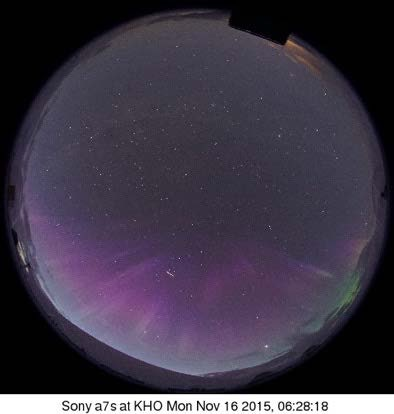
\includegraphics[width=.6\linewidth]{bilder/L4_resonant_scattering.jpg}
    \caption{Resonant scattering at KHO\@. Blue emission at the top part of the auroral curtain at dawn.}\label{fig:L4_resonant_scattering}
\end{figure}

\subsection{Proton aurora}
\begin{enumerate}[\(\bullet \)]
    \item weak {\color{blue}blue} emissions at \SI{4861}{\angstrom} (\(\tn{H}_\beta \)) and {\color{red}red} emission at \SI{6563}{\angstrom} (\(\tn{H}_\alpha \)) as excitations of a neutral hydrogen.
    \item intensity range is between \(50\)--\(\SI{300}{\ray}\)
    \item will look like diffuse aurora since they may get hold of an electron, making them neutral for a while
\end{enumerate}
\begin{align*}
    \tn{X}+\tn{H}^+&\rightarrow \tn{X}^+\tn{H}^*\\
    \tn{H}^*&\rightarrow \tn{H}+h\nu \\
    \tn{H}+\tn{X}&\rightarrow \tn{H}^++\tn{X}+e
\end{align*}

\section{Precipitation patterns}
We divide the energies of the particles into three zones: high, medium and low energy particles. High energy is defined to be \(>\SI{20}{\kilo\electronvolt}\) and we see higher number flux from 4 to 12 MLT\@. Medium energy is defined to be \(0.5\)--\(\SI{20}{\kilo\electronvolt}\) and they are often auroral zone particles with the highest flux on the nightside. Low energy is defined to be \(<\SI{1}{\kilo\electronvolt}\) and the are associated to high flux due to their more direct entry.

The particles entering in the cusps are entering in a minima in the magnetic field between the sunward and tailward field lines, and are therefore most often of lower energy than those entering on the nightside, and hence this is mainly sub-visual precipitation. The cusps are direct entry points of magnetosheath plasma into the atmospheres, and they are located at \(\sim 11\)--\(13\) MLT with a width of \(\sim\SI{1}{\degree}\). \Cref{fig:L4_maps_precipitation_pattern} show a map of precipitation patterns for the dayside of the northern hemisphere
\begin{enumerate}[\(\bullet \)]
    \item {\color{red}cusp}: proton and electron precipitation at low energies
    \item {\color{green}mantle}/{\color{blue}LLBL} (lower latitude boundary layer): soft electron precipitation from the magnetosheath
    \item {\color{cyan}CPS} (central plasma sheet)/{\color{blue!50}BPS} (boundary plasma sheet): medium energy electron precipitation from the plasma sheet
    \item \textcolor{yellow}{\contour{black}{polar rain}}: spatially homogenous electron precipitation at a few hundred \si{\electronvolt} energies
\end{enumerate}
\begin{figure}[t]
    \centering
    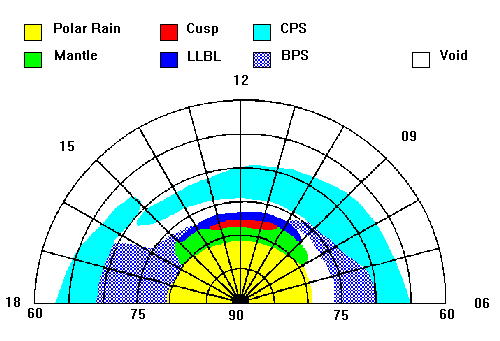
\includegraphics[width=.6\linewidth]{bilder/L4_maps_precipitation_pattern.png}
    \caption{Maps of average precipitation patterns.}\label{fig:L4_maps_precipitation_pattern}
\end{figure}
Some challenges connected to the mapping of precipitation patterns are energy convection and dispersion, field-aligned acceleration and gradient and curvature drifts.

\section{Auroral intensities --- the Rayleigh unit}
For reference, we have that the intensity of the night sky is \(\sim \SI{250}{\ray}\), while the visibility threshold of a human eye is \(\sim \SI{1}{\kilo\ray}\). Auroral intensities are up to \(\sim \SI{1000}{\kilo\ray}\), where the unit \si{\ray} is defined as
\begin{equation}\label{eq:rayleigh_definition}
    \si{\ray}=10^{10}\frac{\tn{photons}}{\si{\metre^2\second}}=4\pi\tn{I}=\int_0^\infty F(\gf{r})\tn{d}r
\end{equation}
where \(F(\gf{r})\) is the volume emission rate. The intensity \(I\) is defined as
\begin{equation*}
    I(X(\lambda))=\frac{\pi}{10^6}\int_0^\infty j(E)P(E)\tn{d}E
\end{equation*}
where \(X(\lambda)\) is a gas \(X\) at a wavelength \(\lambda \), \(E\) is energy, \(j(E)\) is the differential electron or proton energy spectrum and \(P(E)\) is the total number of photons for gas \(X\) at wavelength \(\lambda \). Due to the viewing geometry and the transparency of the aurora, an observer sees surface brightness of the aurora. Rayleigh unit describes this apparent brightness. The distribution of the auroral intensities is shown in \cref{fig:L4_dist_of_auroral_intensities}.
\begin{figure}[t]
    \centering

    \begin{subfigure}[t]{.47\linewidth}
        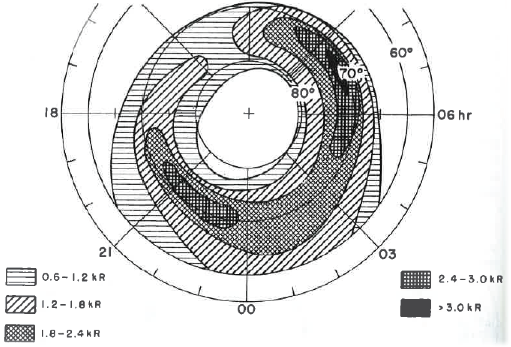
\includegraphics[width=.95\linewidth]{bilder/L4_dist_of_auroral_intensities.png}
        \caption{}\label{fig:L4_dist_of_auroral_intensities}
    \end{subfigure}
    \begin{subfigure}[t]{.47\linewidth}
        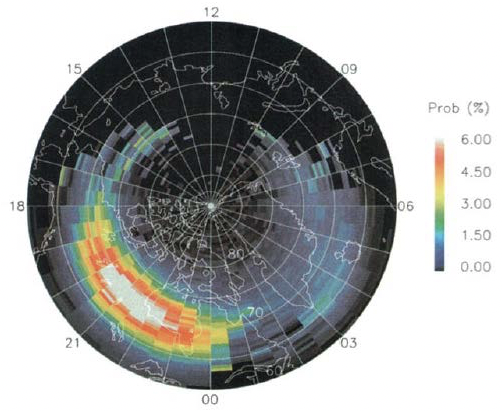
\includegraphics[width=.95\linewidth]{bilder/L4_intensities_darkness.png}
        \caption{}\label{fig:L4_intensities_darkness}
    \end{subfigure}

    \caption{\textbf{\subref{fig:L4_dist_of_auroral_intensities}}: Distribution of auroral intensities. \textbf{\subref{fig:L4_intensities_darkness}}: Intensities as it appears in darkness/light.}\label{fig:L4_intensity_distributions}
\end{figure}

\section{Auroral shapes and forms --- auroral substorms}
\subsection{Currents in the ionosphere}
In order to have currents, we need ion motion relative to the electrons. The velocity difference, and hence current, is strongest in the E-region where the electron motion is governed by \(\gf{E}\times\gf{B}\)-drift and the ion motion is governed by collisions with neutrals.
\(E_x\) --- primary electric field. Continues across the boundary \(\nabla\times\gf{E}=0\). Pedersen: \(\vert\vert E,\perp B\); Hall: \(\perp E,\perp B\). This leads to a more intense current along  the auroral arc. \Cref{fig:L4_E-reg_currents} show the currents in the ionosphere.
\begin{figure}[t]
    \centering
    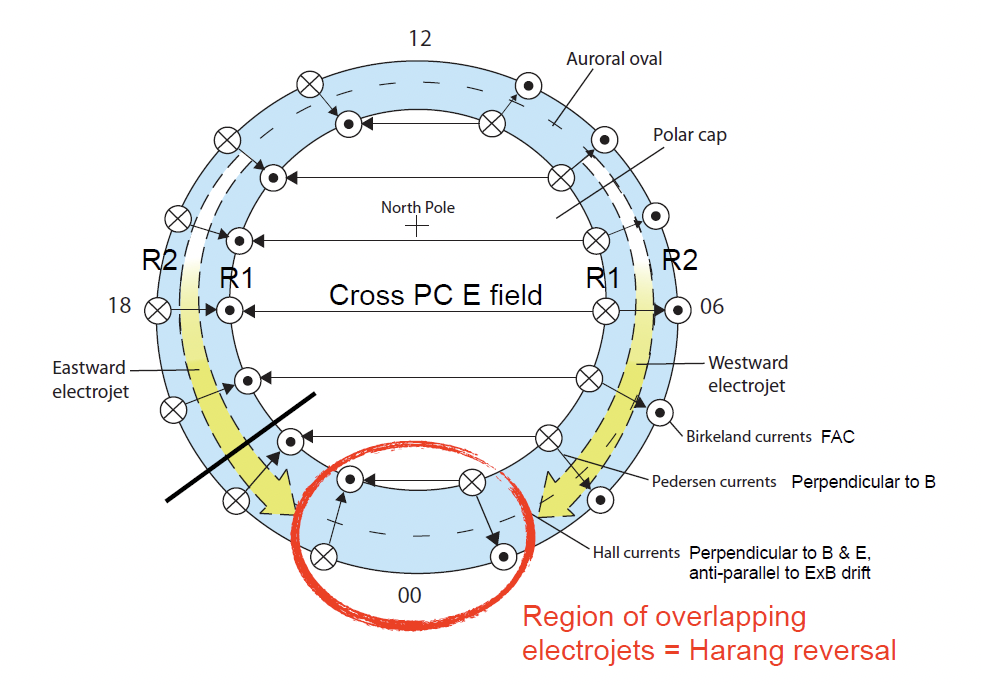
\includegraphics[width=.8\linewidth]{bilder/L4_E-reg_currents.png}
    \caption{Currents in the ionosphere.}\label{fig:L4_E-reg_currents}
\end{figure}
The different forms of aurora can be classified into (1) arcs which is east-west aligned smooth bands with widths of \(\sim 1\)--\(\SI{100}{\kilo\metre}\), (2) rays, magnetic field-aligned small features which often move along the arcs, (3) diffuse/irregular, wide-spread low luminosity distribution which often forms irregular patches of light and (4) vortical structures, spirals, curls, folds and surges, distortions of different sizes along auroral arcs.

Some key features that determine the electrodynamics of auroral structures are the background convection electric field, the relationship between the conductivities inside and outside the aurora and the field-aligned currents associated with the aurora.

The absolute value of the electric field is more intense on the equatorward side than on the poleward side of the arc. The currents of large vortex structures are fed by a converging Pedersen current from the surroundings into an upward field-aligned current. The Hall current around the precipitation region leaves the magnetic trace of upward FAC\@.

\subsection{Polar cap sun-aligned arcs}\label{subsec:sun_aligned_arcs}
This is auroras within the polar cap, pointing towards the sun. They are correlated with IMF \(B_z>0\) and occurs about 50\% of the time. They are of electromagnetic origin and are markers of velocity shear. What we have is a boundary problem, and we either have a flow reversal or a flow gradient. This ends with an electrical field that discontinues across the boundary. In steady state, we must have divergence free currents. In order to get \(\nabla\cdot\gf{j}=0\), a field aligned current is needed. Upward currents are carried by suprathermal electrons, \(E\sim 10-\SI{100}{\electronvolt}\rightarrow \) excitation \(\rightarrow \) light produced.

\subsection{The evolution of substorm aurora}
First, you enter the growth phase, in which quasi-stable arcs are drifting equatorward. The auroral onset often starts equatorward of the preexisting arc and is preceded by the auroral fading. Then comes the expansion phase, and we see auroral madness in multiple forms and scales that are bright and speedy. The last phase is the recovery phase. Here, we find patches, omega-bands and other complicated auroral structures with decaying intensity.
\begin{enumerate}
    \item morphological evolution and description of basic forms
    \item typical location of the substorm onset
    \item extent and speed of the expansion
    \item drift motion and alignments
    \item displays at different parts of the oval
    \item variations in brightness and magnetic field
    \item lifetime of the cycle \(\sim 2\) hours
\end{enumerate}
In MSP data, a substorm would look like an equatorward moving structure during the growth phase, and then followed by a brightening of the equatormost aurora. Next, a rapid poleward expansion of the aurora would fill the field of view. During recovery we see a decay in intensity.

\section{Questions --- week 5}
\begin{enumerate}
    \item [2005 EXERCISE 1]~\\\vspace{-5mm} \begin{enumerate}
        \item \textbf{The aurora can be defined as a three-step process in energy transfer. Discuss briefly the main characteristics of the different energy steps.}\\ First step is an electron that excite an ion. Next we have an ion with potential/chemical energy. At last we see the photon from the emission.
        \item \textbf{List the main phases in an auroral substorm. What characterize the auroras --- intensity, shape and colors --- in the different phases?}\\ The stages are growth (arcs start moving, mostly green), expansion (every color) and recovery (patches, intensity reduces, mostly green).
        \item \textbf{Dayside auroras are very sensitive to the orientation of the interplanetary magnetic field (IMF). Discuss location and dynamics of dayside auroras when:} \begin{enumerate}
            \item \textbf{IMF \(B_z\) is strongly northward}\\ Might reconnect other places, often dependant on \(B_y\)-component. Auroral oval contracts northward. This is when we might see sun-aligned arcs (\cref{subsec:sun_aligned_arcs}).
            \item \textbf{IMF \(B_z\) is pointing southward}\\ Easy reconnection in the equatorial plane. Get auroras on the dayside and nightside with the usual growth, expansion and recovery phases.
        \end{enumerate}
        \item \textbf{An important emission in the night time aurora comes from the following transition:}
        \begin{equation*}
            \tn{OI}~(\prescript{1}{}{S}\rightarrow\prescript{1}{}{D})
        \end{equation*}
        \textbf{Discuss the main characteristics of the emission. Why is quenching by collision important?}\\ This will give green aurora at a wavelength of \(\lambda=\SI{5577}{\angstrom}\). Quenching is important because if quenching is introduced, the ion/molecule will loose its energy before the emission takes place. For this transition, the lifetime is only \SI{0.7}{\second} so you will often see this green light, instead of having its energy being quenched away.
    \end{enumerate}
    \item [2004 EXERCISE 3]~\\\vspace{-5mm} \begin{enumerate}
        \item \textbf{Auroral intensities are usually given in units of Rayleigh [R]. Define the Rayleigh unit in terms of the number of photons hitting the detector. What is a typical value in Rayleighs for the threshold value at 5577 Å for the dark adapted eye?}\\ The definition of the unit can be found in \cref{eq:rayleigh_definition}. Threshold for green is \SI{1}{\kilo\ray}.
        \item \textbf{\Cref{fig:L4_questions} shows daytime auroral intensity measurements obtained using a meridian scanning photometer (MSP). Explain the setup for this instrument, with special care being given to the filters and photo multiplier tube (PMT).}\\ The MSP works by rotating a mirror around an axis perpendicular to the meridian plane with respect to the magnetic north/south, i.e.\ it scans in the meridian plane. Depending on th setting, the MSP will scan for either 8 or 16 s, both peak and base. For an 8 s scan it will spend 4 s rotating once and scan peak values and then the next 4 s to scan base values. A 16 s scan does an average of two scans, i.e.\ two 8 s scans averaged. All four channels in use are measured at the same time. In the MSP are photo multiplier tubes (PMTs). They work as a way of enhancing the sensitivity of the instrument. Its objective is to count photons, and it does so by having an electron potential across its length. The top, where a photon would hit, serves as a cathode, and an electron is knocked loose. Several dynodes along the length of the PMT makes sure the number of electrons that is knocked loose is increasing until they reaches the bottom, where the anode sits. The electrical impulse from the anode is then a measure of how many photons was hitting the cathode.
        \item \textbf{Make a sketch of one of the channels in \cref{fig:L4_questions} showing the cusp region, the open/closed field line boundary and the polar cap region. Also mark clearly which regions are on open and closed field lines.}\\ We use the red channel with wavelength \(\lambda=\SI{6300}{\angstrom}\). From the figure we see the OCB as the lower (equatorward) edge where blue goes to green/red since this is on the dayside. The polar cap would be the upper blue region. The cusp region is then the lower part of the non-blue areas.
        \item \textbf{Other magnetospheric boundary regions include the CPS (central plasma sheet), the LLBL (low-latitude boundary layer) and the Mantle. Describe these three boundary regions with respect to open/closed field lines, energy and flux, as well as the approximate source regions in the magnetosphere (you are free to make a drawing if needed).} \\ Can be found in \cref{fig:L4_maps_precipitation_pattern}. CPS\@: we are on closed field lines, medium to high energy particles, medium to low flux, source is the tail. LLBL\@: boundary between cusp and equatorward. Mantle: on open field lines, low energy particles, medium flux, source is magnetosheath.
        \item \textbf{The 4278 Å \([\tn{N}_2^+1NG]\) (blue) emission line can be used as an indicator for the detection of ionization. Why? What is the average energy loss per collision?}\\ The emission is directly proportional to the energy flux of primary electrons. For one photon, 75 ion pairs are created, and the number of ion pairs created are dependant on the incident energy of the precipitating electron. Therefore, we have a way of going from a measure of how many photons are created to the flux of primary electrons. The average loss per collision is about 36 eV.
        \item \textbf{If \(75\) ion-pairs are produced per photon emitted, estimate the flux needed to produce \(\SI{8}{\kilo\ray}\) of \SI{4278}{\angstrom} emission, given that the mean precipitating energy is \SI{7}{\kilo\electronvolt}.}\\ %Here, I assume that the ratio of the density of nitrogen molecules to the density of the atmosphere is
        % \begin{equation*}
        %     \frac{n(\tn{N}_2)}{n}\approx 0.80
        % \end{equation*}
        Here, I assume that the mean ionization energy is 36 eV. We may find an approximation for the number of photons created by the formula given in \cref{eq:L4_number_of_photons_per_ion}, with the simplification that we only have nitrogen molecules. %This give \(\eta(\SI{4278}{\angstrom})=2.074\). The flux \(\xi \) will then be
        We then get that the flux of photons is \(\num{8e13}\tn{photons}/\si{\metre^{2}\second}\). Multiply this by 75 and you have the flux of ions. For an electron with mean energy \(\varepsilon_0\) we get one ion and loose 36 eV, therefore, the flux \(\xi \) of electrons will be given as
        \begin{equation*}
            \xi=75\cdot 8\cdot 10^{13}\cdot\frac{36}{7000}=\num{30.85e12}\si{\metre^{-2}\second^{-1}}
        \end{equation*}
        % \begin{equation*}
        %     \xi=\num{8000}\cdot 10^{10}\cdot 2.074=\num{165.92e12}\si{\metre^{-2}\second^{-1}}
        % \end{equation*}
    \end{enumerate}
    \item [2007 EXERCISE 1] \textbf{Fast electrons \((e)\) can both ionize and excite gases in the upper atmosphere. These processes can be written symbolically in the following way:}
    \begin{equation*}
        \tn{X}+e\rightarrow {(\tn{X}^+)}^*+e_n+e'
    \end{equation*}
    \textbf{where \(\tn{X}\) is an atmospheric constituent, the asterisk \(*\) indicate that the particle is in an excited state, and \(e_n\) is a thermal electron. In such collisions fast electrons loose in average \SI{35}{\electronvolt}.}
    \begin{enumerate}
        \item \textbf{Where does this energy go? Discuss the energy budget.}\\ One electron is left out (\(e'\)), and then we have the ionization and excitation.
        \item \textbf{If we instead of \(\tn{X}\) use \(\tn{N}_2\), we get:}
        \begin{equation*}
            {\left(\tn{N}_2^+\right)}^*\rightarrow \tn{N}_2^++\left[\SI{3914}{\nano\metre}\tn{ or }\SI{4278}{\nano\metre}\right]\tn{ aurora}
        \end{equation*}
        \textbf{These emissions are called the first negative band system. Why are these bands important in auroral studies?}\\ We can get an estimation of the number of ions in the ionosphere, due to the 25/75 pairs of ions created per photon emitted. We loose \SI{35}{\electronvolt} per ion.
        \item \textbf{Estimate the flux needed to produce \SI{5}{\kilo\ray} of \SI{3914}{\nano\metre} emission, given that the mean precipitation energy is \SI{10}{\kilo\electronvolt}.}\\
        \begin{align*}
            \num{5e13}\tn{ photons/}\si{\metre^2\second}\Rightarrow\num{125e13}\tn{ ions}\\
            35\cdot\num{125e13}\tn{ ions}\rightarrow \num{4375e9}\tn{ electrons/}\si{\metre^2\second}
        \end{align*}
    \end{enumerate}
    \item \textbf{Discuss the excitation mechanism for proton auroras, i.e.\ the hydrogen lines in the auroral spectrum. Why are observations of these emissions so important in space physics?}\\ A proton can pick up an electron to form a fast neutral hydrogen atom, making it free to move across magnetic field lines until a new collision occurs and the atom is stripped of its electron.
    \begin{align*}
        \tn{X}+\tn{H}^+&\rightarrow \tn{X}^++\tn{H}^*\\
        \tn{H}^*&\rightarrow \tn{H}+h\nu \\
        \tn{H}+\tn{X}&\rightarrow \tn{H}^++\tn{X}+e_n
    \end{align*}
    In the neutral state a hydrogen atom can be excited to emit either \(\tn{H}_\alpha \) (6563 Å) or \(\tn{H}_\beta \) (4861 Å). Due to the velocity of an \(\tn{H}^*\) atom along the field line, the wavelengths are Doppler shifted which can be measured, and hence also the velocities of the particles.
    \item \textbf{List the main characteristics of the dayside auroral-oval auroras.}\\ On the dayside there is easier access for the precipitation particles, so intensities can often be lower due to the particles having, on average, lower energy. On the other hand, the flux is higher. This means that for instance the red light, coming from excited states with long lifetimes which for that reason are prone to quenching, have a higher chance of being visible. This makes the dayside aurora appear more red and span a greater range in altitude.
\end{enumerate}
\begin{figure}[ht]
    \centering
    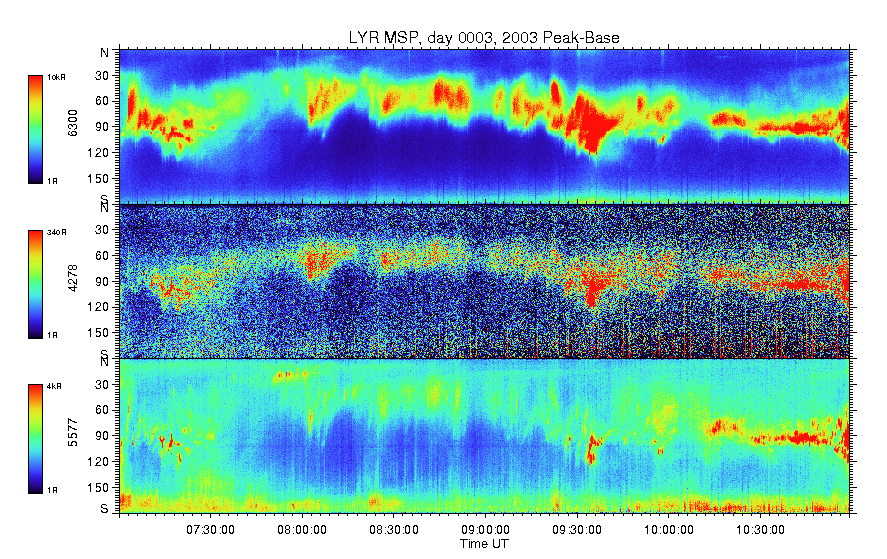
\includegraphics[width=.9\linewidth]{bilder/L4_questions.png}
    \caption{}\label{fig:L4_questions}
\end{figure}